\newpage
\section{Aufbau und Durchführung}\label{sec:aufbau-und-durchfuehrung}
Wie in Abschnitt~\ref{sec:messung} beschrieben, wird zur Messung der Suszeptibilität eine Brückenschaltung wie in Abbildung~\ref{fig:bruecke} benötigt. Um die in Abschnitt~\ref{sec:stoerung} erläuterten Störspannungen zu unterdrücken und die Brückenspannung messen zu können, wird die in Abbildung~\ref{fig:schaltung} gezeigte Schaltung verwendet.

\begin{figure}[H]
 \centering
 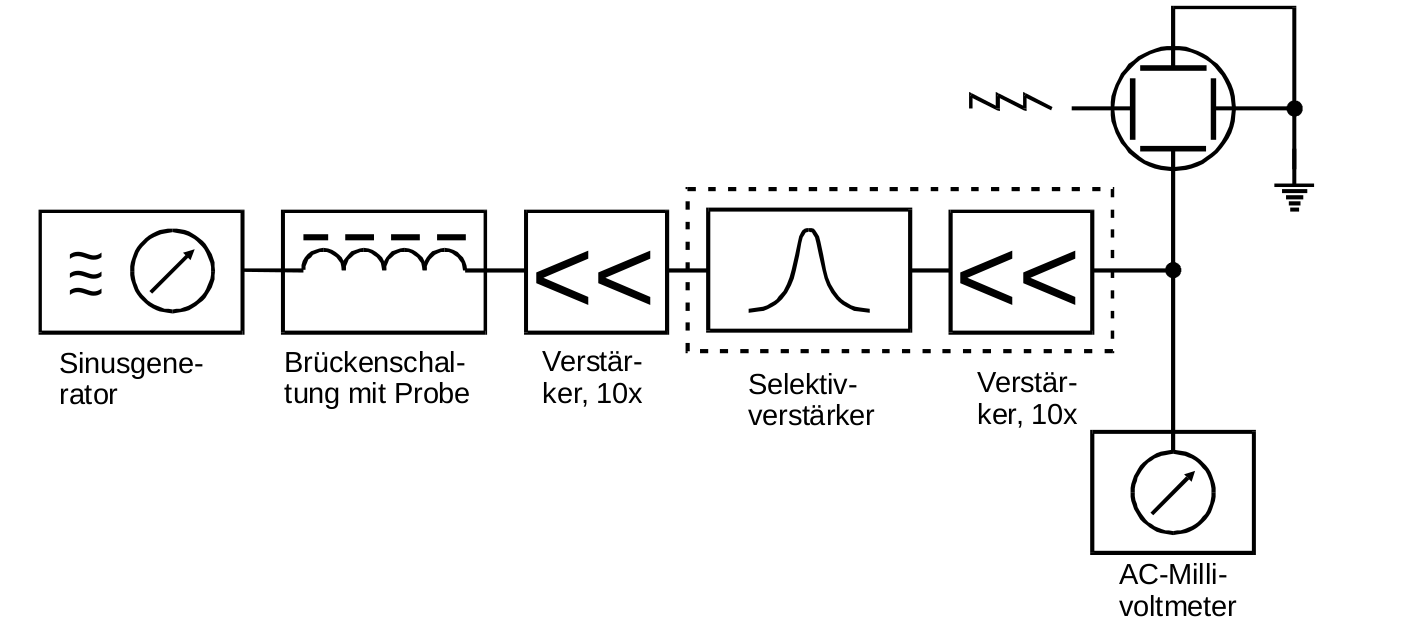
\includegraphics[width=1\textwidth]{../figures/schaltung.png}
 \caption{Schaltbild der zur Messung der Suszeptibilität verwendeten Apparatur.[Skript V606]}
 \label{fig:schaltung}
\end{figure}

Zunächst wird nur der Selektivverstärker bei einer Güte von $Q = 100$ untersucht. Mit Hilfe eines Sinusgenerators wird bei konstanter Eingangsspannung $U_E$ die Ausgangsspannung $U_A$ (am Verstärker) in einem Bereich von 30~-~40~$\si{\kilo\hertz}$ ausgemessen. So lässt sich die Filterkurve des Selektivverstärkers erstellen. Dabei sollte im Bereich der Durchlassfrequenz genauer, also etwa in $\SI{0.1}{\kilo\hertz}$-Schritten, gemessen werden. Aus der Filterkurve kann dann die Durchlassfrequenz ermittelt werden, bei der die Ausgangsspannung maximal wird. Bei dieser Frequenz wird die Messung zur Suszeptibilität durchgeführt, da dort die Störspannungen am besten herausgefiltert werden und die Brückenspannung am genauesten gemessen werden kann.

Nun wird die in Abbildung~\ref{fig:schaltung} dargestellte Schaltung aufgebaut und die Signalfrequenz auf die Durchlassfrequenz des Selektivverstärkers eingestellt, außerdem wird die Speisespannung $U_{Sp}$ notiert.
Mit Hilfe der ersten Methode aus Abschnitt~\ref{sec:messung} wird die Brückenschaltung abgeglichen und die Einstellung des $R_3/R_4$ Widerstandes sowie die -- aufgrund der Störspannungen trotzdem noch -- zu messende Brückenspannung $U_{Br}$ abgelesen. Die Länge der Probe wird ausgemessen, ihre Masse kann einfach abgelesen werden. Daraufhin wird die Probe in einer der Spulen platziert und die Änderung der Brückenspannung wird notiert. Als nächstes wird direkt mit der zweiten Methode weiter gemessen, indem der Widerstand $R_3/R_4$ solange variiert wird, bis die Brückenspannung wieder minimal ist. Auch diese Widerstands-Einstellung wird aufgeschrieben. Die Messung wird für jedes Material dreimal wiederholt. Insgesamt werden drei verschiedene Seltene-Erd-Verbindungen gemessen.

%Der Aufbau ist in Abbildung~\ref{fig:aufbau} zu sehen.
%\begin{figure}[H]
% \centering
% \includegraphics[width=\textwidth]{../figures/aufbau.png}
% \caption{Versuchsapparatur. [Skript V602]}
% \label{fig:aufbau}
%\end{figure}
